\documentclass{beamer}
%\usetheme{Madrid}
%\usetheme{Boadilla}
%\usetheme{default}
%\usetheme{Warsaw}
%\usetheme{Bergen}
%\usetheme{Frankfurt}
\usetheme{Darmstadt}

%\usecolortheme{seahorse}
%\usecolortheme{beaver}
\usecolortheme[named=green]{structure}

\setbeamertemplate{footline}[page number]
%\setbeamercovered{transparent}
\setbeamercovered{invisible}
\setbeamertemplate{navigation symbols}{}

\usepackage{multimedia}
\usepackage{graphicx}
\usepackage[utf8]{inputenc}
%\usepackage[T1]{fontenc}
\usepackage[frenchb]{babel} 
\usepackage[all]{xy}
\usepackage{multirow}
%\usepackage{lmodern}
\usepackage{subfigure}
\usepackage{ulem}
\usepackage{hyperref}

%% --------------

\title[Pr\'esentation C++]{C++, pointeurs et interfaces graphiques}
\author{L\'eo B\textsc{audouin}}
\institute[IFMA]{
  Approfondissement du C++\\
  \medskip
      {\emph{leo.baudouin@ifma.fr}}
}
\date{13 février 2012}

%% --------------

\begin{document}

\begin{frame}
  \titlepage
\end{frame}

\begin{frame}
  \tableofcontents
\end{frame}


\section{Introduction}
\begin{frame}
  Principaux programmes écrits en C ou C++ :
  \begin{itemize}
  \item Windows
  \item Linux
  \item Mac OS
  \item CATIA
  \item Firefox
  \item ...
  \end{itemize}
\end{frame}

\section{Droits d'accès}
\begin{frame}[fragile]{Public, Protected ou Private}

  \begin{small}
\begin{verbatim}
  public : //Accessible partout
    contructeur();
    ~constructeur(); //destructeur
    int variable1;
    void fonction1();
  
  protected : //Accessible dans la classe et les classes filles
    int variable2;
    void fonction2();
  
  private : //Accessible que dans la classe
    int variable3;
    void fonction3();
\end{verbatim}
  \end{small}
\end{frame}
%% --------------

\section{Pointeurs}
\subsection*{Utilisation}
\begin{frame}[fragile]{Les pointeurs}
  \hspace{-12mm}
  \begin{tabular}{l | l | l}
    \begin{minipage}{0.33\linewidth}
      \begin{scriptsize}
\begin{verbatim}
  void fonction(int x)
  {
    x = x + 1;
  }

  void main()
  {
    int a = 1;
    fonction(a);
    printf("a=%d\n",a);
  }
\end{verbatim}
      \end{scriptsize}
    \end{minipage}
    &
    \begin{minipage}{0.33\linewidth}
      \begin{scriptsize}
\begin{verbatim}
  void fonction(int *x)
  {
    *x = *x + 1;
  }

  void main()
  {
    int *a = new int(1);
    fonction(a);
    printf("a=%d\n",*a);
  }
\end{verbatim}
      \end{scriptsize}
    \end{minipage}
    &
    \begin{minipage}{0.33\linewidth}
      \begin{scriptsize}
\begin{verbatim}
  void fonction(int &x)
  {
    x = x + 1;
  }

  void main()
  {
    int a = 1;
    fonction(a);
    printf("a=%d\n",a);
  }
\end{verbatim}
      \end{scriptsize}
    \end{minipage}
  \end{tabular}

  \vspace{5mm}
  
  \begin{block}{
      Que va t'il s'afficher ?}
    \begin{center}
      "a=1" ou "a=2"
    \end{center}
  \end{block}
  
  \pause
  \begin{block}{Réponses}
  1) "a=1" \hfill 2) "a=2" \hfill 3) "a=2"
  \end{block}
\end{frame}

\subsection*{Manipulation de grosses variables}
\begin{frame}[fragile]{Les pointeurs}

  \begin{scriptsize}
    \begin{tabular}{c c}
      \begin{minipage}{0.5\linewidth}
\begin{verbatim}
  class Data{
    void load();
    ...
  };
  int main()
  {
    Data d;
    d.load(); //500Mo
    compute(d);
    return 1;
  }
\end{verbatim}
      \end{minipage}
      &
      \begin{minipage}{0.5\linewidth}
\begin{verbatim}
  class Data{
    void load();
    ...
  };
  int main()
  {
    Data *d = new Data();
    d->load(); //500Mo
    compute(d);
    return 1;
  }
\end{verbatim}
      \end{minipage}
    \end{tabular}
  \end{scriptsize}
    \vspace{2mm}
  \begin{small}
    \begin{block}{Différences}
      Dans le premier cas, la fonction \textit{compute(Data)} doit copier les 500Mo de données en mémoire.\\
      Dans le second cas, la fonction \textit{compute(Data*)} doit copier seulement l'adresse de la variable \textbf{d} (quelques octets) ! 
    \end{block}
    \begin{block}{Attention}
      Les fonctions \textit{compute()} ne prennent pas le même type d'argument.
    \end{block}
  \end{small}
\end{frame}

%------------------------------------------------------------------------------------

\section{Héritage}
\begin{frame}[fragile]{Classe mère / classe fille}
  \begin{scriptsize}
\begin{verbatim}
  class mere {
    ...
  };

  class fille : public mere {
    ...
  };
  
  class cousine : public oncle, tante{
    ...
  }; 
\end{verbatim}
  \end{scriptsize}
\end{frame}

\begin{frame}[fragile]{Classe mère / classe fille}
  \begin{scriptsize}
\begin{verbatim}
  class Vehicule{
    public:
      Vehicule();
      int prix;
  };

  class VehiculeRoulant : public Vehicule{
    public:
      VehiculeRoulant();
      int nombre_roues;
  }

  class Voiture : public VehiculeRoulant {
    public:  
      Voiture();
      string carburant;
  };
\end{verbatim}  
  \begin{block}{Explication}
  L'objet Voiture pourra accéder aux attributs des classes VehiculeRoulant et Vehicule.\\
  Une Voiture aura donc un type de carburant, un nombre de roue et un prix.
  \end{block}
  \end{scriptsize}
\end{frame}

%------------------------------------------------------------------------------------
\section{Polymorphisme}
\subsection*{Polymorphisme 1}
\begin{frame}[fragile]{Polymorphisme}
  \begin{scriptsize}
\begin{verbatim}
  double division(int a, int b)
  {
    printf("Division d'entiers\n");
    return (double)a/(double)b;
  }

  double division(double a, double b)
  {
    printf("Division de doubles\n");
    return a/b;
  }
\end{verbatim}

\begin{block}{Fonctionnement}
Ici la fonction appelée dépend du type de variables passées en arguments. 
\end{block}
  \end{scriptsize}
\end{frame}

\subsection*{Polymorphisme 2}
\begin{frame}[fragile]{Polymorphisme et fonctions virtuelles}
  \begin{scriptsize}
\begin{verbatim}
  class Forme {
    public:
      virtual float aire() = 0;
  };
  
  class Carre : public Forme {
    public:
      virtual float aire() { return cote*cote; }
    private:
      float cote;
  };
  
  class Cercle : public Forme {
    public:
      virtual float aire() { return 3.1415926535*rayon*rayon; }
    private:
      float rayon;
  };
\end{verbatim}

  \end{scriptsize}
\end{frame}

\section{Interfaces Graphiques}
\subsection*{Exemples}
\begin{frame}{Les interfaces graphiques}
  
\includegraphics[width=\linewidth]{images/interface}\\
  \url{https://github.com/lbaudouin/ViewFilmsDataBase}
\end{frame}

\subsection*{QtCreator}
\begin{frame}{QtCreator - Drag and Drop}
  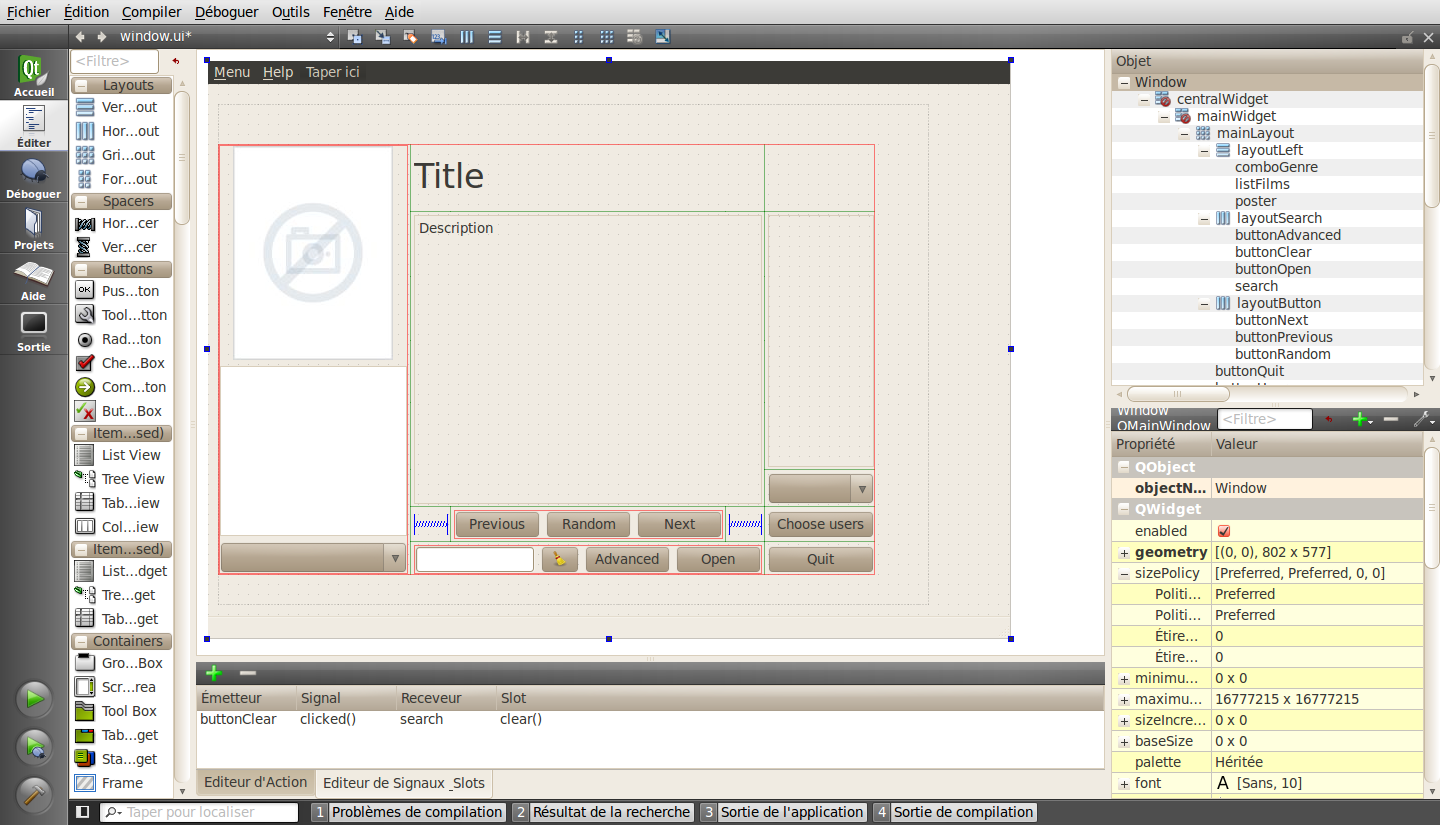
\includegraphics[width=\linewidth]{images/qtcreator}\\
  %\url{https://github.com/lbaudouin/ViewFilmsDataBase}
\end{frame}

\subsection*{Qt}
\begin{frame}[fragile]{Exemple}

  \begin{scriptsize}
    \begin{block}{main.cpp}

\begin{verbatim}
  #include <QtGui/QApplication>
  #include "fenetre.h"

  int main(int argc, char *argv[])
  {
    QApplication a(argc, argv);
    fenetre f;
    f.show();
    return a.exec();
  }
\end{verbatim}
    \end{block}
  \end{scriptsize}


  \begin{block}{Un programme avec Qt}
    - Application\\
    - Fenêtre
  \end{block}
\end{frame}

\begin{frame}[fragile]{Exemple}

  \begin{scriptsize}
  
  \begin{block}{Aide}
  Comme pour le main.cpp, les autres fichiers utiles sont créés et complétés automatiquement par QtCreator !!!
  \end{block}
    \begin{block}{fenetre.cpp}
\begin{verbatim}
  #include "fenetre.h"
  #include "ui_fenetre.h"

  fenetre::fenetre(QWidget *parent) :
    QMainWindow(parent),
    ui(new Ui::fenetre)
  {
    ui->setupUi(this);
  }

  fenetre::~fenetre()
  {
    delete ui;
  }
\end{verbatim}
    \end{block}
  \end{scriptsize}
\end{frame}

\subsection*{Nouveaux types}

\begin{frame}[fragile]%{Nouveaux Types}

  \begin{scriptsize}
    \begin{block}{Signaux et slots à déclarer dans le {\bf .h}}
\begin{verbatim}
  signals:
    void signalSansArgument();
    void signalAvecArgument(int);
  private slots:
    void slotSansArgument();
    void slotAvecArgument(int);
\end{verbatim}
    \end{block}

    \begin{block}{Connections à effectuer pendant l'exécution}
\begin{verbatim}
  connect(this,SIGNAL(signalSansArgument()),
          this,SLOT(slotSansArgument()));
  connect(this,SIGNAL(signalAvecArgument(int)),
          this,SLOT(slotAvecArgument(int)));
\end{verbatim}
    \end{block}
    
    \begin{block}{Signal}
\begin{verbatim}
  emit(signalAvecArgument(2));
\end{verbatim}    
    \end{block}

    \begin{block}{Connections avec l'interface}
\begin{verbatim}
  connect(ui->button,SIGNAL(clicked()),
          this,SLOT(slotSansArgument()));
\end{verbatim}
    \end{block}
  \end{scriptsize}
\end{frame}

\section{Conclusion}
\begin{frame}[fragile]{Trucs et astuces}
  \begin{scriptsize}
    \begin{block}{Langage}
\begin{verbatim}
  x==1?si_vrai:si_faux; //Comme un if
  
  for(int i=0, int j=0; i<10, j<100; j+=i, i++) //Double for
    printf("%d - %d\n",i,j);  
  
  float var1 = 1.5;
  float var2 = (int)var1;	//Conversion de type
  //var2 = 1.0;
  
  #define PI 3.14159265358979323846264338327950288419616939937510
\end{verbatim}
    \end{block}
  \end{scriptsize}
  
  \pause
  \vspace{1cm}
    \begin{center}
    {\huge Bon courage !!!}
    \end{center}
\end{frame}


\end{document}  
